\documentclass[solution, letterpaper]{cs121}

\usepackage{tikz-qtree}
\usepackage{graphicx}
\usepackage{color}
\usepackage{amsfonts}
\usepackage{amsmath}
\usepackage[english]{babel}
\usepackage[utf8]{inputenc}
\usepackage{ae,aecompl}

% allow metapost figures to be included inline
% note: you must invoke latex using:
%
%     pdflatex -shell-escape <inputfile>
%
% to allow it to invoke external commands. See the very end of the
% document as well.
\usepackage{emp,ifpdf}
\usepackage{graphicx}

% convert metapost figures to .eps or .pdf automatically when
% including them
\ifpdf\DeclareGraphicsRule{*}{mps}{*}{}\fi

% include the metapost macros
\empprelude{input boxes; input theory}

%% Please fill in your name and collaboration statement here.
%\newcommand{\studentName}{Renzo Lucioni and Daniel Broudy}
%\newcommand{\collaborationStatement}{I collaborated with...}
\newcommand{\solncolor}{red}
\begin{document}

% create a metapost file for figures to be dumped to.  It's easiest
% to use a single file for all the figures in the document
\begin{empfile}

\header{4}{April 12, 2013, at 12:00 PM}{}{}

%%%%%%%%%%%%%%%%%%%%%%%%%%%%%%%%%%%%%%%%%%%%%%%%%%%%
\problem{14} %1

\subproblem %a
The diagram below illustrates the directed graph structure of the network.

\begin{center}
\begin{emp}(0,0)
  % it's good practice to pick a basic size unit and make all your
  % distances relative to that unit
  u := 2cm;
  ubernodes;
  % create a node, and position its center at the origin
  node.q1(btex $MAI$ etex); q1.c = origin;

  % position the other nodes relative to it
  node.q2(btex $NAI$ etex); q2.c = q1.c + (1.5u,0);
  node.q3(btex $RD$ etex); q3.c = q1.c + (3u,0);
  node.q4(btex $VRAS$ etex); q4.c = q1.c + (0.75u,-1.5u);
  node.q5(btex $SMOS$ etex); q5.c = q1.c + (2.25u,-1.5u);
  node.q6(btex $VP$ etex); q6.c = q1.c + (1.5u,-3u);

  % mark q1 as a start node
  %makestart(q1);

  % mark q4 as an accept node
  %makefinal(q1);

  % draw the nodes
  drawboxed(q1,q2,q3,q4,q5,q6);

  edge(q1,q4,right,btex etex);
  edge(q2,q4,right,btex etex);
  edge(q3,q5,right,btex etex);
  edge(q4,q6,right,btex etex);
  edge(q5,q6,right,btex etex);

\end{emp}
\end{center}

The following describes a parameterization of the noise in the causal effects of the above dependencies.

$P(RD,SMOS,VRAS,MAI,NAI,VP) = 
P(MAI)P(NAI)P(RD)P(VRAS | MAI, NAI)P(SMOS | RD)P(VP | VRAS, SMOS)$\\

Nodes $MAI$, $NAI$, and $RD$ are binary attributes which are not conditional on any other attributes. They are each associated with a probability vector.

\begin{center}
\begin{tabular}{ l |c r }
   $MAI = 0$ & $MAI = 1$ \\
   \hline
  .5 & .5 \\
\end{tabular}
\end{center}

P(VRAS | MAI, NAI)\\
\begin{center}
\begin{tabular}{ l |c r }
   VRAS = 0 & NAI = 0 & NAI = 1 \\
   \hline
  MAI = 0 & .5 & .2 \\
  MAI = 1 & .2 & .1 \\
\end{tabular}
\end{center}

\begin{center}
\begin{tabular}{ l |c r }
   VRAS = 1 & NAI = 0 & NAI = 1 \\
   \hline
  MAI = 0 & 0 & 1 \\
  MAI = 1 & 1 & 1 \\
\end{tabular}
\end{center}


P(SMOS | RD)\\
%SMOS $\in$ \{ 0,1\}\\
%RD $\in$ \{ 0,1\}\\
\begin{center}
\begin{tabular}{ l |c r }
   & RD = 0 & RD = 1 \\
   \hline
  SMOS = 0 & .8 & .2 \\
  SMOS = 1 & .1 & .9 \\
\end{tabular}
\end{center}


P(VP | VRAS, SMOS)\\
\begin{center}
\begin{tabular}{ l |c r }
   VP = 0 & SMOS = 0 & SMOS = 1 \\
   \hline
  VRAS = 0 & .7 & .1 \\
  VRAS = 1 & .1 & .1 \\
\end{tabular}
\end{center}

\begin{center}
\begin{tabular}{ l |c r }
   VP = 1 & SMOS = 0 & SMOS = 1 \\
   \hline
  VRAS = 0 & .1 & .1 \\
  VRAS = 1 & .1 & .7 \\
\end{tabular}
\end{center}

\subproblem %b
 We made the assumption that VRAS and SMOS are independent. We could have plausibly not made this assumption and added an edge from SMOS to VRAS because if you have silly messages on the screen you probably have V-Rases all over the place.  
 
 Another adjustment we could make is to collapse the MAI node and the NAI node because it doesn't really matter if you have more than one virus software, its more important if it you just have Virus software present. 

\subproblem %c

\begin{center}
\begin{emp}(0,0)
  % it's good practice to pick a basic size unit and make all your
  % distances relative to that unit
  u := 2cm;
  ubernodes;
  % create a node, and position its center at the origin
  node.q1(btex $MAI$ etex); q1.c = origin;

  % position the other nodes relative to it
  node.q2(btex $NAI$ etex); q2.c = q1.c + (1.5u,0);
  node.q3(btex $RD$ etex); q3.c = q1.c + (3u,0);
  node.q4(btex $VRAS$ etex); q4.c = q1.c + (0.75u,-2.5u);
  node.q5(btex $SMOS$ etex); q5.c = q1.c + (2.25u,-2.5u);
  node.q6(btex $VP$ etex); q6.c = q1.c + (1.5u,-4u);
  node.q7(btex $VRM$ etex); q7.c = q1.c + (.3u,-1.2u);
  node.q8(btex $VRN$ etex); q8.c = q1.c + (1.2u,-1.2u);

  % mark q1 as a start node
  %makestart(q1);

  % mark q4 as an accept node
  %makefinal(q1);

  % draw the nodes
  drawboxed(q1,q2,q3,q4,q5,q6,q7,q8)

  edge(q7,q4,right,btex etex);
  edge(q8,q4,right,btex etex);
  edge(q3,q5,right,btex etex);
  edge(q4,q6,right,btex etex);
  edge(q5,q6,right,btex etex);
  edge(q1,q7,right,btex etex);
  edge(q2,q8,right,btex etex);

\end{emp}
\end{center}

P(VRM | MAI\\
\begin{center}
\begin{tabular}{ l |c r }
   & VRM = 0 & VRM = 1 \\
   \hline
  MAI = 0 & .1 & .1 \\
  MAI = 1 & 1 & .7 \\
\end{tabular}
\end{center}


P(VRN | NAI\\
\begin{center}
\begin{tabular}{ l |c r }
   & VRN = 0 & VRN = 1 \\
   \hline
  NAI = 0 & .1 & .1 \\
  NAI = 1 & 1 & .7 \\
\end{tabular}
\end{center}


P(VRAS | VRM, VRM)\\
\begin{center}
\begin{tabular}{ l |c r }
   VRAS = 0 & VRN = 0& VRN = 1 \\
   \hline
  VRM = 0 & .5 & .2 \\
  VRM = 1 & .2 & .1 \\
\end{tabular}
\end{center}

\begin{center}
\begin{tabular}{ l |c r }
   VRAS = 1 & VRN = 0 & VRN = 1 \\
   \hline
  VRM = 0 & .1 & .2 \\
  VRM = 1 & .2 & .5 \\
\end{tabular}
\end{center}
We are operating under the assumption that if one virus software reports the other is very likely to have reported as well.

%%%%%%%%%%%%%%%%%%%%%%%%%%%%%%%%%%%%%%%%%%%%%%%%%%%%
\problem{24} %2
\subproblem 
%- For graph (a) I and D are independent of A given knowledge of B. D is conditionally independent because knowledge of B make is independent. I is just always independent of A.\\
- For graph (a) There are no variables that are Independent of A given the knowledge of B\\
%see Reading http://research.microsoft.com/en-us/um/people/cmbishop/prml/Bishop-PRML-sample.pdf 
%page 378.

- For graph (b) only F and C are independent of A given J. In this case we would think the path through G would be blocked because G is is a head to head node. With the knowledge of J, G does not block the path between A and D because J is a decedent node of G, this creates an induced dependence between A and D. This is not the case between D and E, H does not create induced dependence because it is unknown, that being said the existence of B, an unknown tail tail connection, means there is a dependence between D and E. Now finally between E and F we get independence because I is a head-head node and none of its descendants are known. This leaves us with the conclusion that F and C are the only two nodes that are independent of A when J is known. Knowledge of J creates a lot more dependence in this directed graph.

%%%%%%%%%%%%%%%%%%%%%%%%%%%%%%%%%%%%%%%%%%%%%%%%%%%%
\problem{25} %3

% (0.2*NormalDistribution[1, 25]) + (0.3*NormalDistribution[-2, 1])+(0.05*NormalDistribution[3, 4])
\subproblem %a

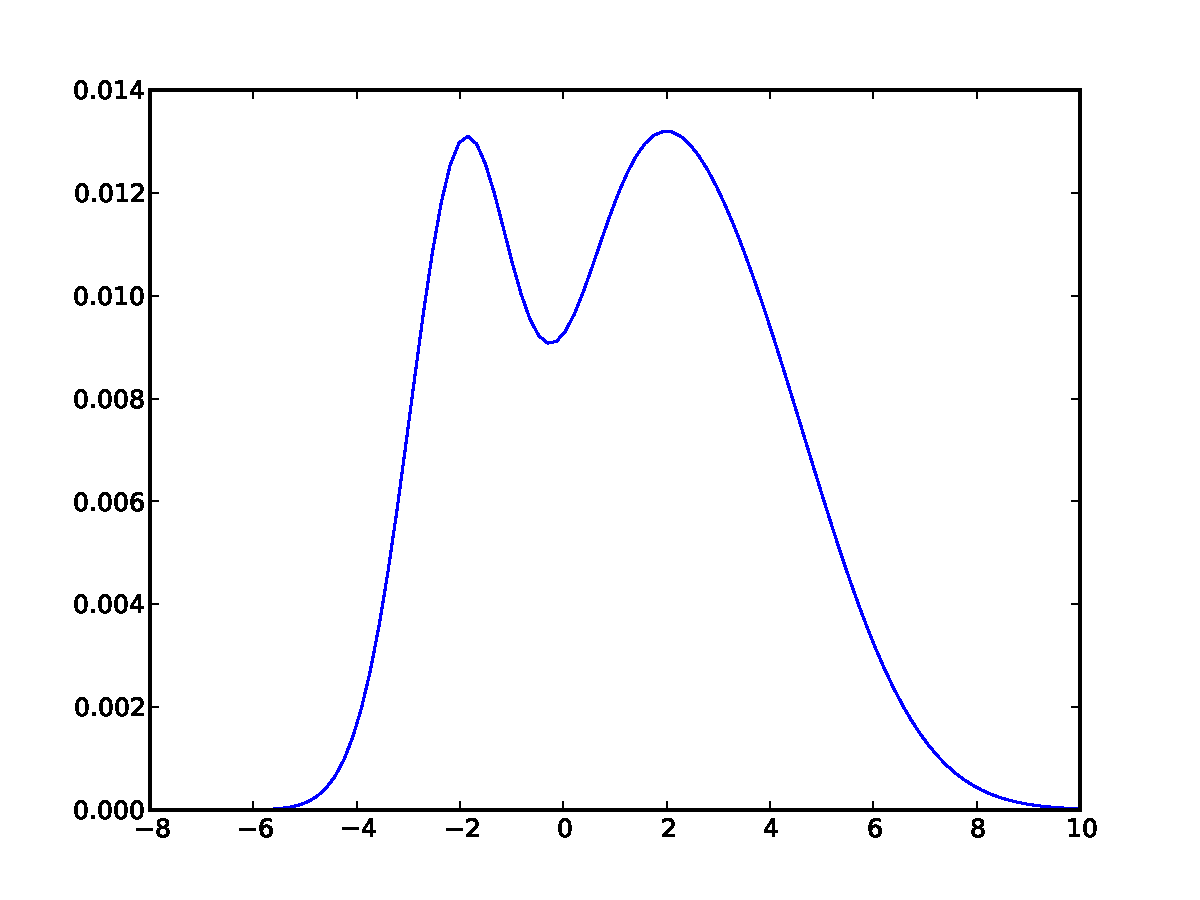
\includegraphics[width=170mm]{mixture_o_gaussians.pdf}

\subproblem %b
To generate data directly from the above distribution, we use the inversion method discussed in class. That is, we assume we have the CDF and inverse CDF of the distribution $f(x)$, then draw a point $u$ uniformly from the vertical axis. We input this point to the inverse of the CDF to get a corresponding value $u'$ on the horizontal axis. We use $u'$ as our sample.

\end{empfile}

% this invokes metapost on the figures. You must run latex a second
% time for the figures to be included.
\immediate\write18{mpost -tex=latex \jobname}

\end{document}






